% ==================================================================
\section{问题三：模态归因与可回溯的局部证据}\label{sec:q3}
% ==================================================================

问题三不再训练新模型，而是在问题二冻结的正式模型 PM-B2 上做解释，这样解释的就是实际做预测的那个模型。解释分三层：模态层用 Shapley 值给出三个模态各起了多大作用；位置层用删除检验找出模型最依赖的词或帧，并检验这些证据是否真的影响输出；素材层把证据位置回指到原词、秒数和帧号，由人工核对。

\subsection{解释对象}

问题三使用 PM-B2 为问题三保存的检查点\todo{注明是否与问题二部署的 seed 17 检查点相同}。完整输入下，模型同时输出三类概率 $\boldsymbol p_i$ 和强度 $\hat y_i$。令
\begin{equation}\label{eq:target}
c_i^\star=\mathop{\arg\max}_{c}\ p_i(c)
\end{equation}
为完整输入下的预测类别。后面所有的分类归因都针对这个固定的 $c_i^\star$，删掉某个模态之后即使预测类别变了，我们看的仍是 $c_i^\star$ 这一类的概率。这样做是为了回答一个确定的问题：“模型之所以判为这一类，各部分分别贡献了多少”，而不是每删一次就换一个问题。附件4没有真值，因此本章报告的是预测的结构和解释的一致性，而不是准确率。

\subsection{模态层：八子集精确 Shapley 值}\label{sec:shap}

设模态集合 $N=\{T,A,V\}$。对任一子集 $S\subseteq N$，构造只保留 $S$ 的输入：$S$ 以外模态的数值和可观测掩码同时关闭。分类与强度的“价值函数”定义为
\begin{equation}\label{eq:value}
v_i^{\mathrm{cls}}(S)=p_i\big(c_i^\star\mid S\big),\qquad v_i^{\mathrm{reg}}(S)=\hat y_i(S).
\end{equation}
空集 $\varnothing$ 返回训练集类别先验和强度中位数，与训练、验证、专项推理时的全空处理一致。按固定顺序枚举 $\varnothing,T,A,V,TA,TV,AV,TAV$ 这8个子集，模态 $m$ 的 Shapley 贡献为
\begin{equation}\label{eq:shap}
\phi_{i,m}^h=\sum_{S\subseteq N\setminus\{m\}}\frac{|S|!\,(2-|S|)!}{3!}\Big[v_i^h\big(S\cup\{m\}\big)-v_i^h(S)\Big],\qquad h\in\{\mathrm{cls},\mathrm{reg}\}.
\end{equation}
它的含义是：把三个模态按所有可能的顺序依次加入，模态 $m$ 加入时带来的输出变化的平均值\cite{lundberg2017shap}。三模态只有8个子集，因此可以精确计算，不需要采样近似。计算用64位浮点，并逐样本检查效率恒等式
\begin{equation}\label{eq:eff}
\Big|\sum_{m\in N}\phi_{i,m}^h-\big[v_i^h(N)-v_i^h(\varnothing)\big]\Big|\le10^{-6}.
\end{equation}
728条验证样本和20条附件4样本的两个输出都通过了这项检查。这只说明分摊的算术是对的，并不说明解释符合人对情绪的理解；后者要靠下一节的删除检验和人工核对。

单条样本的贡献可以为负：如果某一路输入反而降低了预测类别的概率，负值本身就是有意义的解释，我们不对它取绝对值后当成支持证据。每个样本的主导模态取贡献最大的模态，分类和强度分别给出；当 $v_i^h(N)-v_i^h(\varnothing)$ 接近零时，各模态的占比没有意义，我们留空而不强行归一化。此外，我们还在预先选定的96条解释样本上换了一种空集基准做敏感性检查，不同基准下的排序变化单独记录。

图\ref{fig:shap}是验证集728条样本上三个模态的平均绝对贡献。

\begin{figure}[htbp]
\centering
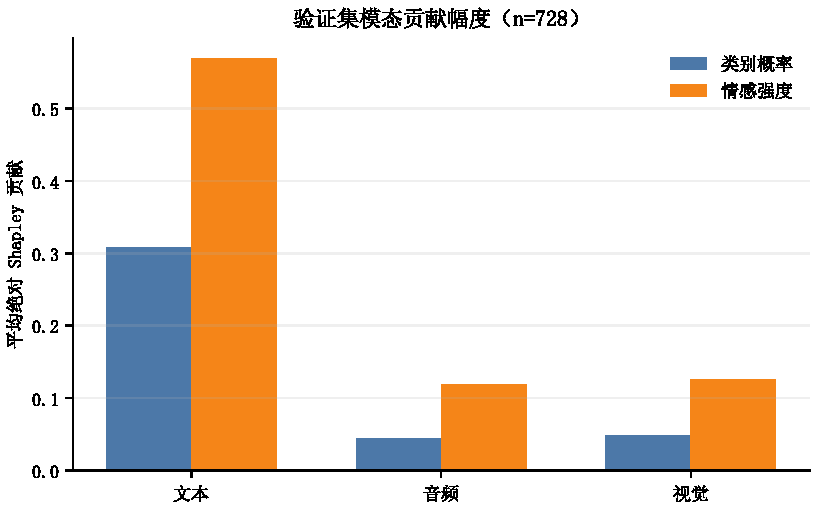
\includegraphics[width=0.66\textwidth]{figures/fig_q3_shapley.pdf}
\caption{验证集728条样本的模态平均绝对 Shapley 贡献（蓝：分类，针对完整输入的预测类别概率；橙：强度输出）}
\label{fig:shap}
\end{figure}

从图中读数，分类输出上文本的平均绝对贡献约为0.31，语音和视觉只有约0.04和0.05，文本是后两者的6～7倍；强度输出上文本约0.57，语音、视觉约0.12和0.13，差距缩小到4～5倍。也就是说，声学和视觉对“有多强烈”的贡献，比对“是正是负”的贡献相对更大。这和直觉一致：语气的轻重、表情的幅度更多反映情感的强弱，而正负方向主要由说了什么决定。这一模态层的结论，也与第\ref{sec:law}节“遮蔽文本是性能下降主因”的结果互相印证。

\subsection{位置层：局部证据与删除检验}\label{sec:local}

先确定解释哪些样本。我们在验证集上按真实类别分层，再对“样本键加固定盐”做 SHA-256 排序，选出96条解释对象。选取过程完全不看模型的预测分数，以免只挑“解释得好看”的样本。

对每个可观测位置，分别删除它的文本、声学或视觉证据，记录目标类概率和强度的变化，作为该位置的局部得分。文本的删除沿用问题二的做法：保留原来的50个位置，把被删的词元换成 PAD 并更新注意力掩码，再经冻结的 BERT 重新编码，而不是把缓存的 BERT 向量置零；声学、视觉则在原位置关闭可观测掩码并重新标准化。令 $R_k$ 为局部得分最高的前 $k$ 个位置，定义
\begin{equation}\label{eq:del}
C_{i,k}^{\mathrm{cls}}=p_i\big(c_i^\star\mid N\big)-p_i\big(c_i^\star\mid N\setminus R_k\big),\qquad
S_{i,k}^{\mathrm{cls}}=p_i\big(c_i^\star\mid N\big)-p_i\big(c_i^\star\mid R_k\big).
\end{equation}
$C$ 衡量删掉这些证据后目标类概率下降多少，越大说明证据越关键；$S$ 衡量只保留这些证据时损失多少，越小说明这几处证据越“够用”\cite{deyoung2020eraser}。强度输出同时保存有符号和绝对值的变化。作为对照，用同样的预算删除得分最低的位置和随机位置；随机位置重复20次，在每个样本内部取平均，这20次是同一样本内的对照，不算20个独立样本。附件4上的结果见图\ref{fig:faith}。

\begin{figure}[htbp]
\centering
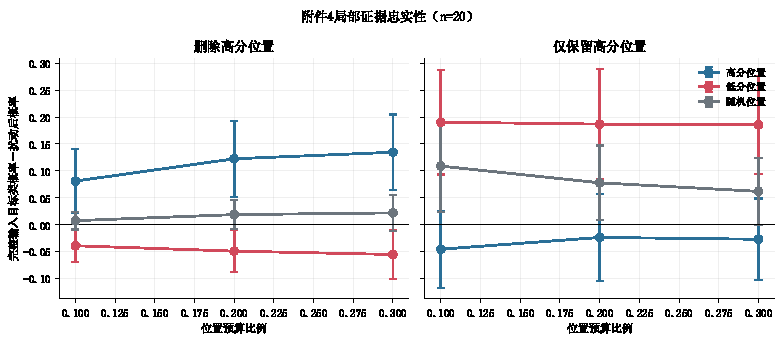
\includegraphics[width=\textwidth]{figures/fig_q3_faithful.pdf}
\caption{附件4（20条）分类证据的删除检验（左）与保留检验（右）。横轴为位置预算占可观测位置的比例；纵轴为完整输入的目标类概率减去扰动后的概率；误差线为20条样本之间的标准差}
\label{fig:faith}
\end{figure}

左图中，三条线分得很开。删除得分最高的位置，目标类概率的下降随预算增加而增大，预算为30\%时平均约0.14；删除随机位置只下降约0.03；删除得分最低的位置，概率反而略有上升（约 $-0.05$），说明这些位置本来是在“拉低”预测类别。右图中，只保留高分位置时概率损失最小（接近0甚至为负），只保留低分位置时损失最大。两张图的方向一致，说明局部得分确实抓住了模型所依赖的位置。不过误差线较宽，20条样本之间的差异不小；而且这些差值说明的是“模型怎么用这些位置”，并不能直接当作这些词在情感上的因果证据。

\subsection{素材层：人工时间核验}\label{sec:review}

局部证据回指到原素材时，用的是问题一建立的“子词位置—词—秒数—帧号”反查链。附件4的人工核验表共有1662个“词—模态”映射行，其中1599行通过、63行被拒绝，被拒绝的63行全部来自样本15：人工核对后确认它的文字与声音对不上，强制对齐给出的时间不可信。另外，样本02从第5个位置起的45行时间整体偏移，按核验结果统一修正了 $-0.55$ 秒。

对样本15，我们保留模型预测和与时间无关的 Shapley 值、删除得分，但从最终展示的时间映射、证据表和解释卡中清除这63行的起止秒数和帧号，只在审计字段里保留工具的原始输出。因此，其余19条可以给出核验过的时间，样本15只给出位置级的解释。模型层面的忠实性检验和素材层面的人工核验是两件事：前者回答“模型是不是这么用的”，后者回答“视频里是不是真有这个”，谁也不能代替谁。

\subsection{附件4的预测与解释}\label{sec:att4}

附件4的20条样本全部输出了三类概率、强度、两个输出的模态贡献和局部证据，逐条汇总见附录\ref{app:C}的表\ref{tab:appC}，分布见图\ref{fig:special}(b)。

20条中正向10条、负向7条、中性3条，平均类别概率为0.717；其中4条（09、10、11、16）强度低于 $-1.5$，是比较强烈的负向，置信度都在0.93以上。分类的主导模态以文本为主（16条），其余为视觉3条（02、05、14）和声学1条（13）；强度的主导模态文本17条、视觉3条（01、05、14）。把两个输出合起来看，有一个很清楚的规律：分类或强度任一输出以非文本为主导的5条样本（01、02、05、13、14），类别概率都不超过0.565，平均只有0.497；两个输出都以文本为主导的15条，平均为0.790。也就是说，当模型主要靠声音或画面做判断时，它自己也没那么有把握。这些样本正是最值得人工回看的。

题目要求给出典型样本的解释卡。以样本01为例，解释卡见表\ref{tab:card}。

\begin{table}[htbp]
\centering
\caption{解释卡示例：附件4样本01}
\label{tab:card}
\begin{tabularx}{\textwidth}{l>{\raggedright\arraybackslash}X}
\toprule
项目 & 内容 \\
\midrule
预测极性与强度 & 中性；强度 $+0.137$（精确值0.1368） \\
三类概率 & 负向0.1154，中性0.5162，正向0.3684 \\
主要参考模态 & 分类：文本；强度：视觉 \\
模态作用程度 & 分类 $\phi^{\mathrm{cls}}_{T},\phi^{\mathrm{cls}}_{A},\phi^{\mathrm{cls}}_{V}=$ \todo{从解释 CSV 抄录}；强度 $\phi^{\mathrm{reg}}_{T},\phi^{\mathrm{reg}}_{A},\phi^{\mathrm{reg}}_{V}=$ \todo{从解释 CSV 抄录} \\
文本关键证据 & Replacing（0.501–0.942 s），timing（2.726–3.007 s）等；对应子词位置 \todo{位置号} \\
声学、视觉证据 & 与上述词时间窗对应的声学帧与视频帧 \todo{视频帧号} \\
时间核验 & 人工核验通过 \\
读法 & 分类主要依据文本，但文本没有把预测推向明确的正负（中性0.52对正向0.37）；强度的主导模态是视觉，给出的是轻微的正值 \\
\bottomrule
\end{tabularx}
\end{table}

这张卡说明了一个有代表性的情况：两个输出头的主导模态不同。分类主要看文本，而“Replacing”“timing”这类词本身没有明显的情感倾向，分类落在中性也就不奇怪；强度则主要由视觉决定，结果是一个轻微的正值。这里的词时间是原素材上的定位，不是这个词单独的情感标签。

题目还要求展示主导模态内局部片段的重要性分布。图\ref{fig:localimp}给出样本01在文本模态上逐位置的局部得分。

\IfFileExists{figures/fig_q3_local_importance.pdf}{%
\begin{figure}[htbp]
\centering
\includegraphics[width=\textwidth]{figures/fig_q3_local_importance.pdf}
\caption{附件4样本01文本模态的逐位置局部得分（横轴为子词位置，标注原词）}
\label{fig:localimp}
\end{figure}}{%
\begin{figure}[htbp]
\centering
\fbox{\parbox{0.9\textwidth}{\centering\vspace{1.2cm}\todo{用解释 CSV 中样本01文本模态的逐位置局部得分画柱状图（横轴子词位置并标注原词），保存为 figures/fig\_q3\_local\_importance.pdf 后重新编译}\vspace{1.2cm}}}
\caption{附件4样本01文本模态的逐位置局部得分}
\label{fig:localimp}
\end{figure}}

\subsection{错误归因}\label{sec:q3err}

\textbf{（1）解释会如实暴露模型对文本的依赖。}绝大多数样本以文本为主导，这是模型真实的行为，解释只是把它说了出来。反过来看，如果某条样本的转写有错，模型大概率会跟着错，而解释卡上会写着“文本主导”，读者据此就知道应该先核对转写。

\textbf{（2）非文本主导的样本置信度偏低。}第\ref{sec:att4}节的5条样本类别概率都不超过0.565，其中样本02只有0.380，基本处在“猜”的状态。对这类样本，解释给出的主导模态本身也不太稳定，更适合作为“请人工复核”的提示，而不是结论。

\textbf{（3）证据时间受强制对齐质量限制。}样本15的文字与声音对不上，时间全部作废；样本02有整体0.55秒的偏移。1662行中有108行（6.5\%）需要拒绝或修正，说明自动对齐的时间不能不经核对就直接当证据用。

\textbf{（4）删除检验的差异在样本间波动较大。}图\ref{fig:faith}的误差线较宽，低预算时高分位置曲线的下沿已接近随机位置，说明样本之间差异不小。20条样本的结论在方向上是清楚的，但幅度还需要更多样本来确认。

\subsection{小结}

问题三在不改动模型的前提下，从模态、位置、素材三层给出了解释。精确 Shapley 值的效率恒等式在全部样本上成立；删除检验显示高分位置确实比随机位置更影响预测；人工核验拒绝了不可信的时间，而没有为它们编造秒数。附件4的20条中，以非文本为主导的样本置信度明显偏低，这为人工复核提供了一个简单实用的筛选依据。
